\newpage
\section{Ergebnisse}
In diesem Kapitel werden die zentralen Ergebnisse der Arbeit präsentiert. 
Schwerpunkt ist der entwickelte \acs{aas}-Demonstrator für die robocell, gefolgt von der Analyse des eingesetzten Modells zur Anomalieerkennung und einer Diskussion weiterer \acs{ki}-Anwendungen. 
Anschließend werden die beiden Anwendungsfälle \acs{dpp} und automatisierte Generierung der \acs{aas} vorgestellt. 
Den Abschluss bildet eine Bewertung der im Projekt eingesetzten Softwarelösungen und Tools.

\subsection{AAS-Demonstrator für die robocell}
Für das Abfüll- und Verschließmodul der robocell wurde ein digitaler Zwilling auf Basis der \acs{aas} entwickelt.  
Der Demonstrator kombiniert standardisierte Templates der \acs{idta} mit individuell angepassten Submodellen und wurde als konkrete Instanz modelliert, um Echtzeitdaten anzubinden und praxisnahe Anwendungsfälle darzustellen.
Die entwickelte Struktur kann dabei als Vorlage für zukünftige Projekte dienen.  
Die verwendeten Daten erheben keinen Anspruch auf Vollständigkeit, sondern dienen in erster Linie der exemplarischen Demonstration.

Im Folgenden wird zunächst die Systemarchitektur des Demonstrators aufgezeigt.  
Darauf aufbauend erfolgt ein Überblick über den strukturellen Aufbau, bevor die enthaltenen Submodelle im Detail vorgestellt werden.  
Diese gliedern sich in statische Submodelle zur Abbildung von Stammdaten sowie in dynamische Submodelle zur Erfassung von Zustands- und Prozessdaten.

\subsubsection{Systemarchitektur}
Die Architektur des Demonstrators basiert vollständig auf containerisierten Komponenten, die innerhalb einer gemeinsamen Docker-Umgebung organisiert sind.
Dies ermöglicht eine modulare und skalierbare Infrastruktur, die sich flexibel erweitern und anpassen lässt.
Als zentrale Plattform zur Verwaltung und Bereitstellung der \acs{aas} wurde Eclipse BaSyx eingesetzt.
Ursprünglich war der Einsatz des AASX Server Blazor vorgesehen, dieser wurde jedoch frühzeitig durch BaSyx ersetzt, da es eine deutlich flexiblere und umfassendere Umgebung für digitale Zwillinge bietet.

Die vollständige Systemarchitektur ist in Abbildung~\ref{fig:Systemarchitektur} dargestellt.
Sie unterstützt die Integration sowohl statischer als auch dynamischer Submodelle, die Kommunikation über standardisierte Schnittstellen sowie die Anbindung von Echtzeit- und Zeitreihendaten.
\acs{aas}-spezifische Daten werden dabei in einer MongoDB persistiert, während Zeitreihendaten in einer InfluxDB gespeichert werden.

\begin{figure}[htbp]
    \centering
        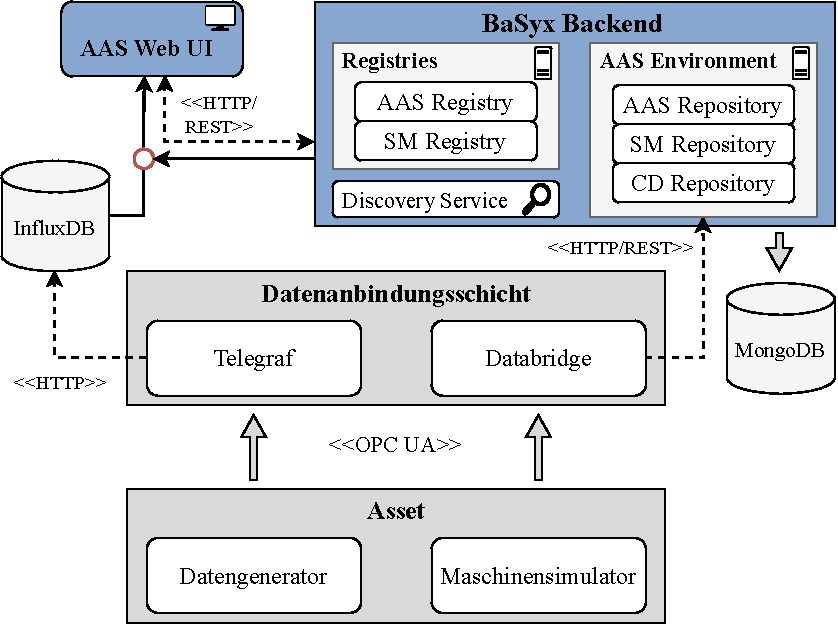
\includegraphics[width=1\textwidth]{Bilder/Ergebnisse/DynamischeDaten/Architektur.pdf}
    \caption{Systemarchitektur AAS-Demonstrator}
    \label{fig:Systemarchitektur}
\end{figure}

% Eine weitere, in der Abbildung nicht dargestellte Komponente ist ein als Docker-Container ausgeführtes Node.js-Skript, das beim Start der BaSyx-Umgebung automatisch fehlende Einträge im Discovery Service anlegt.
% Hierzu werden relevante Asset-Informationen aus einer JSON-Datei ausgelesen und in den Service eingetragen.
% Diese Funktionalität ist insbesondere für die Abbildung hierarchischer Strukturen sowie für den Anwendungsfall der PCF-Berechnung im Rahmen des \acs{dpp} von Bedeutung.

Ein wesentlicher Vorteil der gewählten Architektur besteht darin, dass sich die AAS Web UI jederzeit durch alternative Frontends oder zusätzliche Services ersetzen lässt.
Dadurch können sowohl eigene Anwendungen als auch externe Softwarelösungen flexibel integriert werden.
Im Rahmen dieser Arbeit wurde beispielsweise alternativ der Mnestix Browser eingesetzt, der eine vergleichbare Funktionalität wie die AAS Web UI bietet \cite{Quelle}.
Eine detaillierte Evaluierung dieses Werkzeugs erfolgt in Kapitel~\ref{ref}.

\subsubsection{Aufbau und Metadaten}

+ Metadaten des Assets und der AAS zB bilder von PE
+ Modellierung untergeordneter komponenten mit eigener AAS
+ Wie QR Code bei groninger. Gibt es nichtr nicht es wurde beispiel id verwendet um das umzusetzten an die MAaschine euiien Code mit der Asset ID
+ Wenn man den scanntn kommt man dahin

\subsubsection{Stammdaten}

Die statische Modellierung der \acs{aas} und ihrer Submodelle erfolgte ausschließlich mit dem Package Explorer. 
Sämtliche Stammdaten der Maschine wurden dabei manuell eingepflegt.
Als Hauptdatenquellen für die statischen Informationen dienten die technische Dokumentationen der robocell, insbesondere die Betriebsanleitung, sowie Informationen aus dem \acs{plm}-System Agile.

\subsubsection*{Typenschild}
\vspace{-0.5em}

Das Submodell Typenschild bildet die zentrale Identifikationsstelle eines Assets innerhalb der \acs{aas} und entspricht funktional einem physischen Typenschild. 
Es enthält grundlegende Informationen wie Hersteller, Seriennummer oder Produkttyp. 
Auch bei Maschinen von groninger sind solche Typenschilder vorhanden, jedoch meist reduziert auf die wichtigsten Angaben.

Die digitale Variante innerhalb der \acs{aas} erlaubt eine erweiterte Darstellung dieser Informationen, die sowohl maschinenlesbar als auch interoperabel sind. 
Dazu zählen beispielsweise Softwareversionen, Zertifikate, Logos, Kontaktinformationen oder weitere produktspezifische Angaben, die über ein physisches Typenschild hinausgehen. 

Das Typenschild zählt zu den wichtigsten Submodellen und ist daher auch als Plugin in der AAS Web UI verfügbar. 
Dort ist es unterteilt in Produktinformationen und Herstellerinformationen. 
In Abbildung~\ref{fig:typenschild-ui} ist exemplarisch der Herstellerbereich des Plugins dargestellt.

\begin{figure}[htbp]
    \centering
        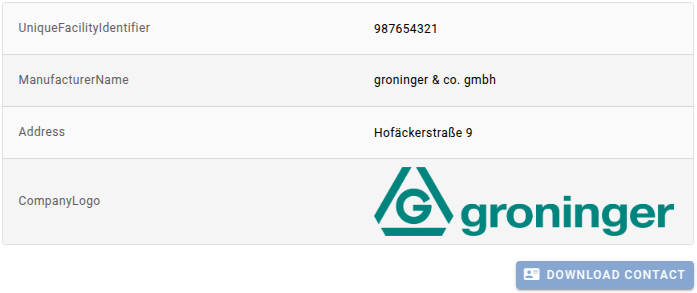
\includegraphics[width=1\textwidth]{Bilder/Ergebnisse/StatischeDaten/Typenschildisualisierung.png}
    \caption{Metadatenstruktur im Submodell Dokumentation}
    \label{fig:Doku}
\end{figure}

\subsubsection*{Technische Daten}
\vspace{-0.5em}


\subsubsection*{Dokumente und 3D-Modelle}
\vspace{-0.5em}
Im Submodell Dokumentation werden alle relevanten Unterlagen zur Maschine und ihren Komponenten gepflegt.
In dieser Arbeit wurden exemplarisch Dokumente wie die Betriebsanleitung, Funktionsspezifikationen, eine Netzwerkübersicht sowie die Projektzeichnung eingebunden.
Diese sind als File-Elemente direkt in die \acs{aas}-Struktur eingebettet.

Allerdings umfasst die Dokumentation mehr als nur das Einfügen von Dateien.
Jedes Dokument ist in einer eigenen \acs{smc} organisiert, die dem \acs{smt} HandoverDocumentation \cite{SpezifikationDokumentation} folgt.
Darin sind strukturierte Metadaten wie eine eindeutige Dokumentenkennung, Klassifikation und Versionsinformationen hinterlegt.
Abbildung \ref{fig:Doku} zeigt die Metadatenstruktur am Beispiel der Funktionsspezifikationen.

\begin{figure}[htbp]
    \centering
        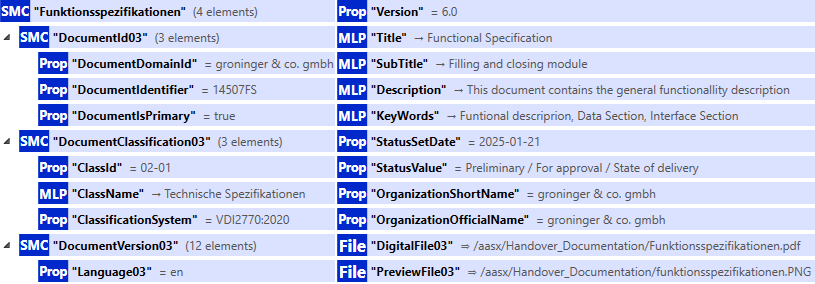
\includegraphics[width=1\textwidth]{Bilder/Ergebnisse/StatischeDaten/Doku.png}
    \caption{Metadatenstruktur im Submodell Dokumentation}
    \label{fig:Doku}
\end{figure}

Die gezeigte Struktur ist universell einsetzbar und kann für beliebige Dokumenttypen verwendet werden, so auch für 3D-Modelle.
Zwar existiert mit dem \acs{smt} Provision of 3D-Models \cite{Spezifikation3DModelle} ein speziell dafür vorgesehenes, deutlich umfangreicheres Template, dessen Aufbau der Dokumentationsstruktur ähnelt, jedoch zusätzliche Felder wie die geometrische Beschreibung oder Darstellungsoptionen enthält.
In der Praxis stellt sich jedoch die Frage, ob der zusätzliche Aufwand zur vollständigen Umsetzung dieses Templates gerechtfertigt ist, insbesondere dann, wenn die dafür benötigten Daten nicht vollständig vorliegen oder nicht gepflegt werden.
Aus diesem Grund wurde in dieser Arbeit auf eine vereinfachte Struktur zurückgegriffen, die sich an der Dokumentationslogik orientiert.

Sowohl Dokumente als auch 3D-Modelle lassen sich über entsprechende Plugins in der AAS Web UI (Typ-2-\acs{aas}) sowie im Package Explorer (Typ-1-\acs{aas}) visualisieren und herunterladen.
Dies ermöglicht eine einfache Nutzung und einen direkten Zugriff auf die eingebundenen Inhalte.

\subsubsection*{Hierarchische Strukturen}
\vspace{-0.5em}
Das \acs{bom}-Submodell dient der Darstellung hierarchischer Strukturen innerhalb des \acs{aas}-Demonstrators.
Die Idee in dieser Arbeit war es, exemplarisch die Stückliste der Maschine abzubilden, nicht vollständig, sondern anhand einer Auswahl relevanter Komponenten.
Jede dieser Komponenten wurde als eigenständige \acs{aas} modelliert, wodurch eine modulare und erweiterbare Struktur entsteht.

Abbildung \ref{fig:BOM} zeigt die hierarchische Struktur diese Submodells.
Im Zentrum befindet sich das Submodell der Haupt-\acs{aas}, das die erste untergeordnete Ebene abbildet.
Links und rechts sind jeweils referenzierte Komponenten-\acs{aas} dargestellt, die über Entity-Elemente mit dem Submodell der Haupt-\acs{aas} verknüpft sind.

\begin{figure}[htbp]
    \centering
        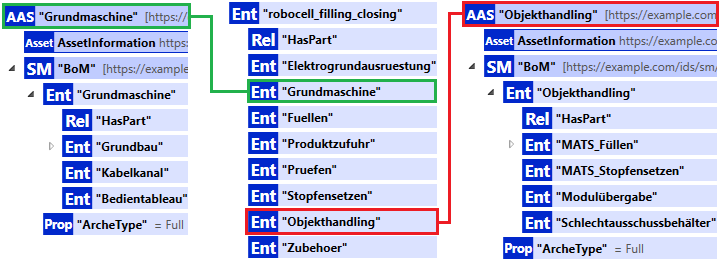
\includegraphics[width=1\textwidth]{Bilder/Ergebnisse/StatischeDaten/BOM.png}
    \caption{Systemarchitektur AAS-Demonstrator}
    \label{fig:BOM}
\end{figure}

Die einzelnen Komponenten sind als Self-Managed Entities modelliert, da sie jeweils über eine eigene \acs{aas} verfügen.
Die Referenzierung erfolgt dabei über die globalAssetId, wodurch eine direkte Verbindung zur jeweiligen Komponente hergestellt wird.

Zur Abbildung der Beziehungen zwischen den Komponenten wird ein RelationshipElement verwendet.
Primär kommt dabei die Beziehung HasPart zum Einsatz, deren Bedeutung über eine zugewiesene semanticId eindeutig beschrieben ist.
Auf diese Weise lässt sich die Struktur einer Maschine rekursiv modellieren: Jede Komponente kann wiederum über ein eigenes \acs{bom}-Submodell verfügen, in dem weitere Unterkomponenten referenziert sind.

Die AAS Web UI bietet ein Plugin zur Visualisierung dieser Beziehungen. 
In der grafischen Oberfläche werden die HasPart-Beziehungen zwischen den Komponenten visuell dargestellt. 
Abbildung \ref{fig:BOMVisualisierungUI} zeigt ein Beispiel der Grundmaschine, bei dem wiederum die erste untergeordnete Ebene abgebildet ist.

\begin{figure}[htbp]
    \centering
        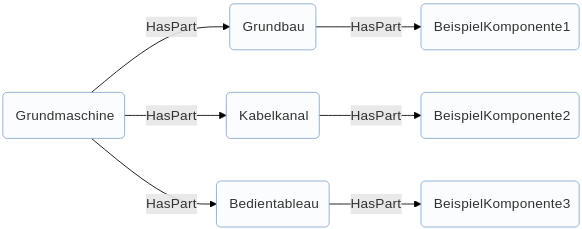
\includegraphics{Bilder/Ergebnisse/StatischeDaten/BOMVisualisierungUIpng.png}
    \caption{BOM-Visualisierung der Grundmaschine in der AAS Web UI}
    \label{fig:BOMVisualisierungUI}
\end{figure}

Wird eine untergeordnete Komponente innerhalb der Visualisierung selektiert, erfolgt eine direkte Navigation zur zugehörigen \acs{aas}. 
Diese Verlinkung basiert auf der globalAssetId und setzt voraus, dass die entsprechende Komponente im Discovery Service registriert ist. 
Dort ist für jede Komponente ein Eintrag hinterlegt, der die globalAssetId mit der eindeutigen ID der jeweiligen \acs{aas} verknüpft. 
Die AAS Web UI nutzt diese Informationen, um die entsprechende \acs{aas} automatisch aufzulösen und in der Benutzeroberfläche anzuzeigen.

\subsubsection*{Wartung}
\vspace{-0.5em}
Das Submodell Wartung bildet den digitalen Wartungsplan der robocell-Maschine ab. 
Es enthält strukturierte Informationen zu einzelnen Komponenten, darunter der letzte Wartungszeitpunkt, das Wartungsinterval, die zuständige Person oder Organisation sowie die durchzuführenden Maßnahmen. 
Diese Informationen sind für jede Komponente in einer \acs{smc} organisiert.

Sofern die \acs{aas} über eine geeignete Plattform wie Eclipse BaSyx bereitgestellt wird, besteht die Möglichkeit, Wartungsmaßnahmen direkt in der AAS zu erfassen und in den Wartungsplan einzutragen. 
Bedienpersonal sowie interne oder externe Wartungsteams könnten über entsprechende Schnittstellen oder Benutzeroberflächen Einträge vornehmen, wodurch eine nachvollziehbare Dokumentation aller Wartungsaktivitäten gewährleistet wird.

Abbildung \ref{fig:Wartung} zeigt exemplarisch die Wartungsinformationen für zwei Komponenten des Füllmoduls.

\begin{figure}[htbp]
    \centering
        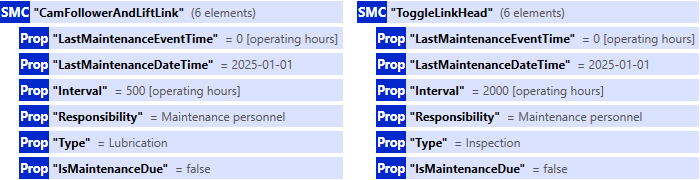
\includegraphics[width=1\textwidth]{Bilder/Ergebnisse/StatischeDaten/Wartung.png}
    \caption{Systemarchitektur AAS-Demonstrator}
    \label{fig:Wartung}
\end{figure}

Das Submodell wurde so entworfen, dass es künftig dynamisch erweitert werden kann. 
Beispielsweise könnte ein Betriebsstundenzähler angebunden werden. 
Eine entsprechende Logik oder ein Skript könnte dann den aktuellen Wert mit dem letzten Wartungszeitpunkt vergleichen und automatisch den Wartungsbedarf erkennen. 
In jeder \acs{smc} wurde dafür eine Property implementiert, die über ein Boolean-Feld angibt, ob eine Wartung fällig ist.

\subsubsection{Zustands- und Prozessdaten}
Die rein statisch modellierte \acs{aas} bildet lediglich die Struktur und Metadaten der robocell-Maschine ab und erfüllt damit noch nicht die Anforderungen an einen digitalen Zwilling gemäß der in Kapitel \ref{sec: DT} dargestellten Klassifizierung. 
Erst durch die Integration von Echtzeitdaten sowie der Möglichkeit zur Interaktion mit dem physischen System entsteht eine digitale Repräsentation, die über eine reine Beschreibung hinausgeht.

Die Erweiterung der \acs{aas} um dynamische Daten wurde in dieser Arbeit durch die Umsetzung von drei Submodellen realisiert, die nachfolgend vorgestellt werden. 
Diese wurden zunächst im Package Explorer strukturiert und anschließend zur Laufzeit in der BaSyx-Umgebung mit simulierten Daten befüllt bzw. aktualisiert.

\subsubsection*{Prozessdaten}
\vspace{-0.5em}

Im Submodell Prozessdaten werden simulierte Werte für Füllstand, Durchfluss, Anzahl abgefüllter Einheiten sowie Druck erfasst.
Diese stammen vom Datengenerator und werden im Sekundentakt erzeugt.
In realen Anwendungen sind jedoch deutlich kürzere Intervalle üblich.
Die kontinuierliche Erfassung und Übertragung der Daten in das Submodell erfolgt über die Databridge, wobei ein Subscription-Modell verwendet wird.
Dadurch werden Änderungen nahezu in Echtzeit in das Submodell überführt.

Die Rohdaten werden zunächst mithilfe des Jackson-Transformers in ein JSON-Objekt transformiert.
Anschließend erfolgt die Extraktion der relevanten Werte mithilfe von JSONata, bevor diese in die entsprechenden Properties des Submodells geschrieben werden.
Genauer gesagt werden die Werte im Submodel Repository der AAS Environment aktualisiert.

Die Werte können über die AAS Web UI visualisiert werden, entweder über die klassische Elemente-Ansicht oder über ein speziell entwickeltes Plugin.
Zur Aktualisierung bietet die Anwendung zusätzlich die Möglichkeit, eine Synchronisation zu aktivieren.
Dabei werden alle relevanten \acs{aas}-Daten in einem definierten Intervall automatisch von den zugrunde liegenden Services abgefragt und anschließend in der Benutzeroberfläche dargestellt.
Die Anzeige der Prozessdaten erfolgt somit nicht in Echtzeit, sondern in regelmäßigen Abständen, beispielsweise alle vier Sekunden, und unabhängig von der tatsächlichen Erzeugungs- oder Übertragungsfrequenz der Daten durch den Datengenerator bzw. die Databridge.

% \begin{figure}[htbp]
%     \centering
%         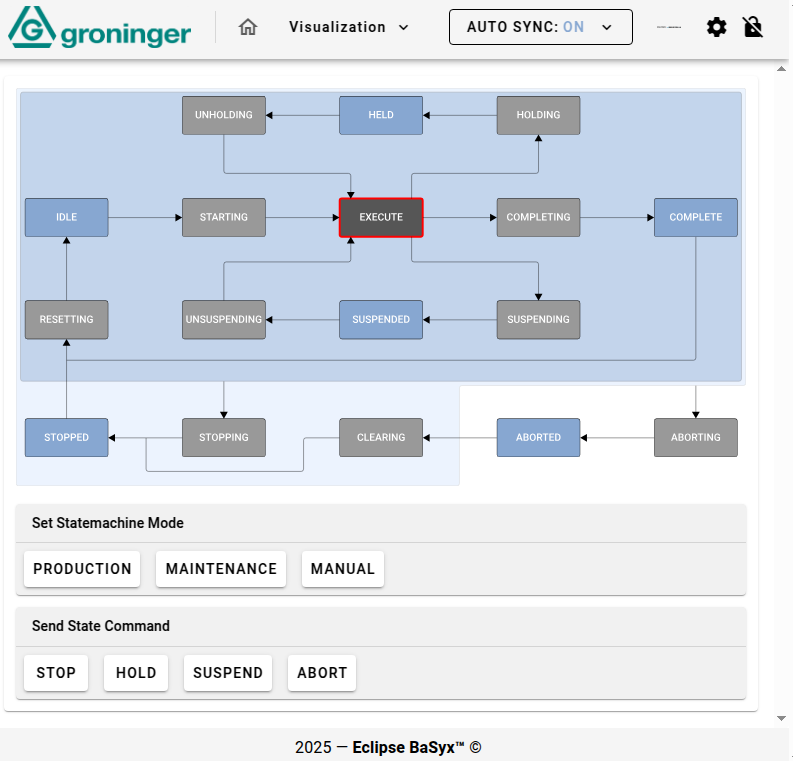
\includegraphics{Bilder/Ergebnisse/DynamischeDaten/ProcessData/Visualisierung.png}
%     \caption{Systemarchitektur AAS-Demonstrator}
%     \label{fig:Systemarchitektur}
% \end{figure}

Der implementierte Mechanismus zur Datenintegration ist protokolloffen und lässt sich flexibel auf verschiedene Kommunikationsprotokolle wie \acs{mqtt} oder \acs{rest} anwenden.
Eine automatisierte Anbindung externer Datenquellen ist somit problemlos möglich.
Aktuell sind die Datenflüsse jedoch primär darauf ausgelegt, Daten von externen Quellen in die \acs{aas} zu übertragen.
Eine Rückführung von Daten aus der \acs{aas} in externe Systeme, beispielsweise über \acs{opcua}, ist bislang noch nicht umgesetzt.

\subsubsection*{Kontrollkomponente}
\vspace{-0.5em}
Ein vergleichbarer Mechanismus wie bei den Prozessdaten kommt auch im Submodell Kontrollkomponente zum Einsatz. 
Die mithilfe des Maschinensimulators generierten Zustandsdaten werden über \acs{opcua} abgefragt und mithilfe der Databridge in das zugehörige Submodell der \acs{aas} geschrieben. 
Da der Simulator numerische Zustände liefert, erfolgt zunächst eine semantische Umwandlung mittels JSONata, um diese in sprechende Zustandsbezeichnungen wie Execute, Stopped oder Suspending zu überführen.

Die Zustände orientieren sich am PackML-Standard, der insgesamt 17 definierte Maschinenzustände umfasst. 
Diese standardisierte Struktur ermöglicht eine konsistente Erfassung und Interpretation des Maschinenstatus und wird auch für die robocell-Linie eingesetzt.
Der Maschinenstatus selbst ist in einer \acs{smc} organisiert, in der eine Property den aktuellen Zustand abbildet.

Zur Visualisierung wurde ein bestehendes Vue.js-Plugin verwendet, das ursprünglich im Rahmen eines Forschungsprojekts an der Hochschule für Technik und Wirtschaft Berlin entwickelt wurde \cite{HTW1}\cite{HTW2}. 
Da das Plugin nicht weiter gepflegt wurde, wurde es funktional angepasst und in die AAS Web UI integriert, um es für den Demonstrator nutzbar zu machen.

Die aktuellen Zustandsinformationen werden darin visuell in Form eines PackML-Zu\-standsautomaten dargestellt, wie Abbildung \ref{fig:PackMLZustandsautomat} zeigt. 
Um Änderungen direkt anzuzeigen, wurde eine Polling-Logik implementiert, die den Maschinenstatus in regelmäßigen Abständen vom Submodel Repository der AAS Environment abfragt.

\begin{figure}[htbp] 
    \centering 
        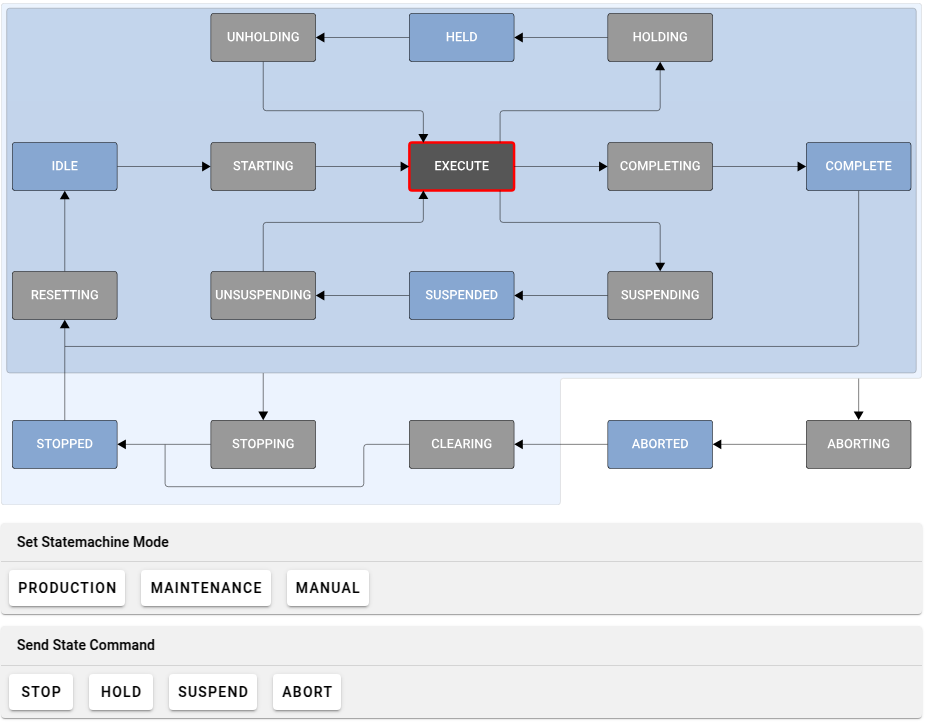
\includegraphics[width=1\textwidth]{Bilder/Ergebnisse/DynamischeDaten/Kontrollkomponente/PackMl.PNG} 
    \caption{Plugin Submodell Kontrollkomponente} 
    \label{fig:PackMLZustandsautomat} 
\end{figure}

Wie auch in der Abbildung zu erkennen besteht neben der Visualisierung auch die Möglichkeit, den Maschinenmodus direkt über die AAS Web UI zu ändern. 
Über interaktive Schaltflächen können Nutzer konforme Zustandsübergänge gemäß PackML auslösen. 
Befindet sich die Maschine beispielsweise im Zustand Execute, sind die Befehle Stop, Hold, Suspend und Abort möglich. 
Nicht erlaubt wären direkte Übergänge zu Zuständen wie Idle, Reset oder Completed.

Zusätzlich kann der Maschinenmodus gesetzt werden. 
Die vorliegende Umsetzung unterstützt drei Betriebsmodi: Produktion, Manuell und Wartung. 
Diese werden analog zum Maschinenstatus über eine entsprechende Property im Submodell Kontrollkomponente im Submodel Repository der AAS Environment verwaltet.

Im Demonstrator wird der Maschinenzustand direkt über eine WebSocket-Verbindung vom Plugin an den Maschinensimulator übermittelt und ohne weitere Prüfung übernommen. 
Dadurch entsteht eine einfache Feedback-Schleife zwischen Benutzeroberfläche und Simulator, die eine direkte Steuerung aus der \acs{aas} ermöglicht.

In einer realen Maschinenumgebung würde der Steuerbefehl zunächst mit einem geeigneten Industrieprotokoll wie \acs{opcua} an die speicherprogrammierbare Steuerung (SPS) der Maschine übertragen werden müssen. 
Nach erfolgreicher Validierung und der Durchführung notwendiger Operationen, etwa dem Abschalten von Motoren oder dem Schließen von Ventilen, würde der neue Zustand gesetzt und anschließend an die \acs{aas} zurückgemeldet werden.

\subsubsection*{Zeitreihendaten}
\vspace{-0.5em}
Das dritte Submodell, das ebenfalls als dynamisches Submodell eingeordnet werden kann, ist die Darstellung von Zeitreihendaten. 
Datengrundlage bilden erneut die simulierten Prozesswerte des Datengenerators.
Diese werden kontinuierlich über Telegraf in eine InfluxDB geschrieben und stehen somit für zeitbasierte Auswertungen zur Verfügung.

Die AAS Web UI ermöglicht den direkten Zugriff auf diese Daten. 
Über die im Submodell hinterlegten Parameter kann eine gezielte Abfrage an die Datenbank gestellt werden. 
Die Ergebnisse werden anschließend im Visualisierungsbereich der Benutzeroberfläche dargestellt. 
Hierzu muss ein Nutzer lediglich das gewünschte Segment sowie die darzustellenden Messgrößen auswählen.

% Wie in Abbildung \ref{fig:KonfigurationZeitreihen} zu erkennen, muss hierzu das gewünschte Segment sowie die darzustellenden Messgrößen ausgewählt werden.
% \begin{figure}[htbp]
%     \centering
%         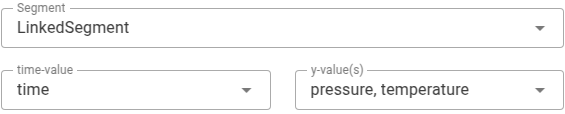
\includegraphics{Bilder/Ergebnisse/DynamischeDaten/ZeitreihenDaten/Konfiguration.png}
%     \caption{Zeitreihendaten in der AAS Web UI}
%     \label{fig:KonfigurationZeitreihen}
% \end{figure}

Zur Visualisierung stehen verschiedene Diagrammtypen zur Verfügung. 
Die Datenbankabfrage selbst ist im LinkedSegment hinterlegt und definiert den Zeitraum, über den die Daten abgefragt werden.
Unabhängig davon kann der Zeitraum, der in der Visualisierung angezeigt wird, individuell angepasst werden.

Abbildung \ref{fig:LiniendiagrammBaSyx} zeigt die Darstellung von Druck und Temperatur über einen Zeitraum von fünf Minuten in einem Liniendiagramm.

\begin{figure}[htbp]
    \centering
        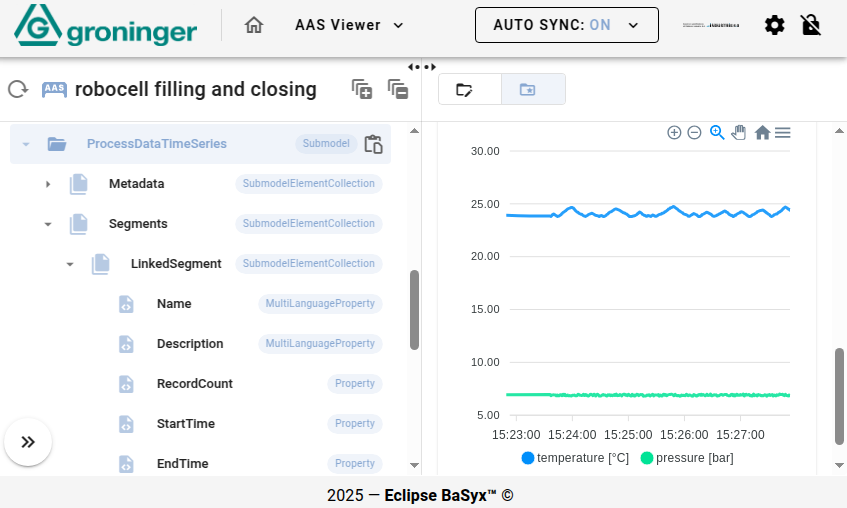
\includegraphics{Bilder/Ergebnisse/DynamischeDaten/ZeitreihenDaten/Liniendiagramm.png}
    \caption{Zeitreihendaten in der AAS Web UI}
    \label{fig:LiniendiagrammBaSyx}
\end{figure}

Ein wesentlicher Vorteil dieser Umsetzung ist die Entkopplung der Datenspeicherung von der \acs{aas} selbst. 
Da die \acs{aas} keine Datenbank ist, eignet sich dieser Mechanismus besonders für die Integration großer oder historischer Datenmengen. 
Er lässt sich flexibel auf beliebige Datensätze anwenden und erweitert so die Funktionalität der \acs{aas} sinnvoll um zeitbasierte Analyse- und Visualisierungsoptionen.

Dabei enthält das Submodell alle notwendigen Informationen, um auch außerhalb der AAS Web UI verwendet zu werden.
Die darin definierten Parameter und Abfragebeschreibungen ermöglichen externen Anwendungen einen gezielten Zugriff auf die zugrunde liegenden Zeitreihendaten.
Das Submodell dient somit als standardisierte Schnittstelle zur Datenbereitstellung und kann für weiterführende Anwendungen wie Analyse-Tools, Monitoring-Systeme oder KI-basierte Verfahren, wie in dieser Arbeit zur Anomalieerkennung demonstriert, genutzt werden.

%KI-Modell
\subsection{Evaluation des KI-Modells}
\subsubsection{Bewertung des prototypischen KI-Einsatzes}
\subsubsection{Ausblick: Predictive Maintenance}
\subsubsection{Weiterführende Einsatzmöglichkeiten}

% Digitaler Produktpass
\newpage
\subsection{Anwendungsfall Digitaler Produktpass}
\subsubsection{Abbildung des PCF}
Zur Abbildung des \acs{pcf} der Gesamtmaschine wurde ein Mechanismus in der AAS Web UI integriert. 
Im Visualisierungsbereich wurde eine Schaltfläche implementiert, über die die Aggregation der CO\textsubscript{2}-Äquivalente ausgelöst werden kann. 
Beim Betätigen dieser wird eine \acs{http}-GET-Anfrage an den Microservice gesendet, der die Berechnung durchführt.

Der Microservice, der ebenfalls als Docker-Container implementiert wurde, reagiert auf die Anfrage und startet den Berechnungsprozess. 
Der Ablauf ist in Abbildung \ref{fig:SequenzdiagrammPCF} als Sequenzdiagramm dargestellt.

\begin{figure}[htbp]
    \centering
        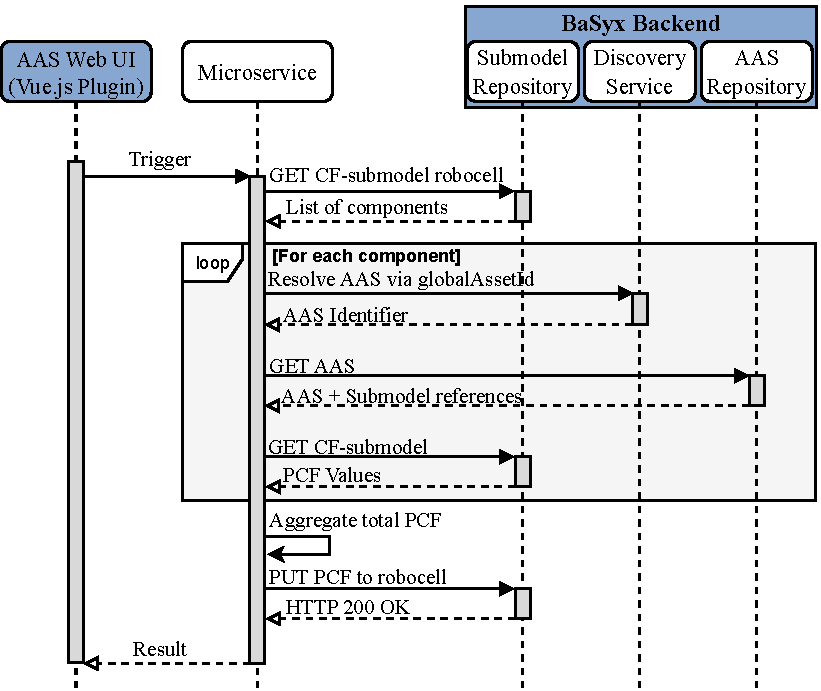
\includegraphics[width=1\textwidth]{Bilder/Ergebnisse/DPP/AggregationNue.pdf}
    \caption{Sequenzdiagramm zur Aggregation des PCF}
    \label{fig:SequenzdiagrammPCF}
\end{figure}

% \begin{figure}[htbp]
%     \centering
%         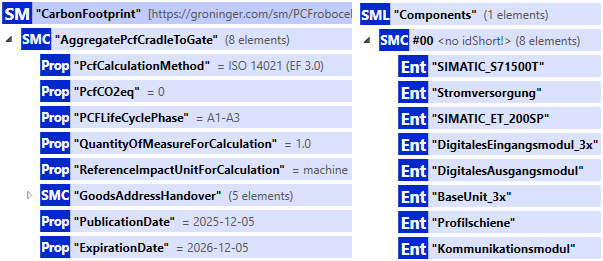
\includegraphics[width=1\textwidth]{Bilder/Ergebnisse/DPP/SubmodellCF.png}
%     \caption{Sequenzdiagramm zur Aggregation des PCF}
%     \label{fig:SequenzdiagrammPCF}
% \end{figure}

Der Microservice nutzt die \acs{rest}-Schnittstelle des Submodel Repositories der AAS Environment, um zunächst alle in der Komponentenliste des \acs{cf}-Submodells der robocell hinterlegten Komponenten auszulesen. 
Mithilfe des Discovery Service werden auf Basis ihrer globalAssetIds die zugehörigen Komponenten-\acs{aas} identifiziert und anschließend vom AAS Repository abgerufen.
Für jede dieser Komponenten wird geprüft, ob ein \acs{cf}-Submodell vorhanden ist. 
Falls dies zutrifft, wird das Submodell ausgelesen und die enthaltenen \acs{pcf}-Werte extrahiert.

Aus den ermittelten Einzelwerten berechnet der Microservice die aggregierten CO\textsubscript{2}-Äquivalente für die Phasen Produktion, Material sowie Cradle to Gate. 
Die berechneten Werte werden abschließend in das \acs{cf}-Submodell der Haupt-\acs{aas} der robocell geschrieben und stehen dort strukturiert zur Verfügung.

Nach Abschluss der Berechnung sendet der Microservice eine Bestätigung an das Plugin zurück. 
Dieses reagiert darauf, indem es das aktualisierte \acs{cf}-Submodell über die \acs{rest}-Schnittstelle der AAS Environment erneut abfragt. 
Die relevanten Submodellelemente werden dabei herausgefiltert und in der Benutzeroberfläche aktualisiert. 
Dadurch werden die aggregierten \acs{pcf}-Werte unmittelbar sichtbar, ohne dass ein manuelles Neuladen erforderlich ist.

Abbildung \ref{fig:PluginAggregation} zeigt die entsprechende Visualisierung. 
Auf der linken Seite sind die berechneten CO\textsubscript{2}-Äquivalente dargestellt, auf der rechten Seite die zugehörigen Lebenszyklusphasen.

\begin{figure}[htbp]
    \centering
        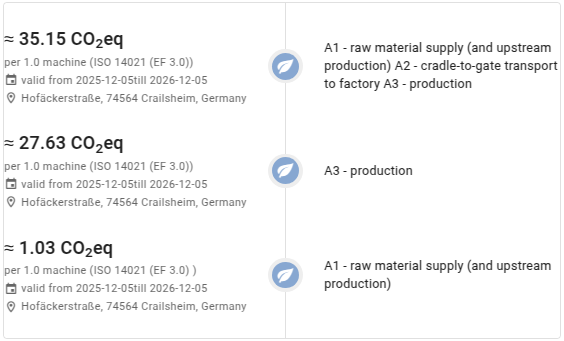
\includegraphics{Bilder/Ergebnisse/DPP/PluginAggregation.png}
    \caption{Visualisierung der aggregierten PCF-Werte im Plugin}
    \label{fig:PluginAggregation}
\end{figure}

Die beschriebene Lösung ermöglicht es, den \acs{pcf} dynamisch auf Basis der in der Komponentenliste referenzierten Steuerungselemente zu berechnen. 
Auch wenn derzeit nur acht Siemens-Komponenten berücksichtigt werden, lässt sich die Liste bei Verfügbarkeit weiterer Komponenten-\acs{aas} unkompliziert erweitern, sodass sukzessive die gesamte Maschine in die Berechnung einbezogen werden kann.

Perspektivisch lässt sich die Berechnung zudem um weitere Lebenszyklusphasen wie Nutzung oder Entsorgung ergänzen, um eine ganzheitliche Betrachtung von der Herstellung bis zum Lebensende eines Produkts bzw. einer Maschine zu ermöglichen.
Darüber hinaus könnte auch der \acs{tcf} berücksichtigt werden, beispielsweise im Rahmen der Auslieferung einer Maschine, wodurch eine noch umfassendere Bilanzierung der Umweltauswirkungen ermöglicht wird.

\subsubsection{Rollenbasierter Zugriff auf Submodelle}
Eine Möglichkeit, die im \acs{dpp} enthaltenen Informationen einzusehen, bietet die AAS Web UI. 
Ist \acs{rbac} aktiviert, wird der Benutzer beim Aufruf der Oberfläche zur Keycloak-Anmeldeseite weitergeleitet. 
Wie in Abbildung \ref{fig:KeycloakAnmeldeSeite} dargestellt, kann sich der Nutzer dort mit dem in Keycloak hinterlegten Benutzernamen und Passwort authentifizieren.

\begin{figure}[htbp]
    \centering
        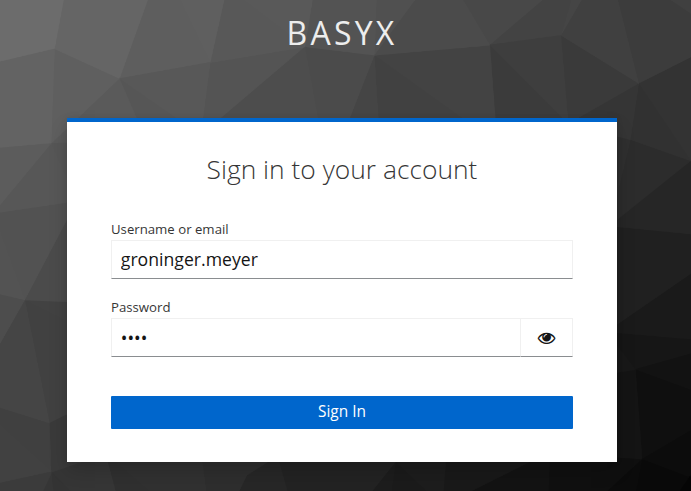
\includegraphics[width=0.7\textwidth]{Bilder/Ergebnisse/DPP/KeycloakAnmeldeSeite.png}
    \caption{Keycloak-Anmeldeseite für die AAS Web UI}
    \label{fig:KeycloakAnmeldeSeite}
\end{figure}

Nach erfolgreicher Anmeldung erhält der registrierte Client (AAS Web UI) ein Zugriffstoken, das die Rolleninformationen des Nutzers enthält.  
Dieses Token wird im Hintergrund an die angebundenen BaSyx-Komponenten (z.\,B. AAS Environment, Registries) weitergegeben.  
Die Entscheidung über die tatsächliche Zugriffsberechtigung trifft dabei nicht die AAS Web UI, sondern der jeweilige Service, indem er die im Token enthaltenen Rollen gegen die hinterlegten RBAC-Regeln prüft.
Ist keine Konfiguration hinterlegt, werden keine AAS angezeigt.

Meldet sich beispielsweise der Benutzer customer.doe an, so sieht er zwar den \acs{dpp}, jedoch nur die Submodelle, die in den RBAC-Konfigurationsdateien für die Rolle Kunde freigegeben sind. 
Dazu zählen beispielsweise das Typenschild, Technische Daten oder der \acs{cf}. 
Andere Submodelle wie 3D-Modelle oder Wartungsinformationen werden nicht angezeigt und erscheinen als nicht gefunden. 
Darüber hinaus besitzt der Benutzer lediglich Leserechte, sodass keine Änderungen an den Inhalten vorgenommen werden können. 
Versucht er, eine neue \acs{aas} über die Benutzeroberfläche hochzuladen, wird der Vorgang mit einem \acs{http}-Fehler 403 abgelehnt.

Neben dem Zugriff über die AAS Web UI ist auch ein direkter Zugriff auf die BaSyx-Komponenten über die \acs{api} möglich.
Dies ist insbesondere für technische Clients oder externe Anwendungen relevant, die automatisiert auf die im \acs{dpp} enthaltenen Informationen zugreifen sollen.
In diesem Fall muss ein Zugriffstoken aktiv über den Token-Endpunkt des entsprechenden Realms in Keycloak angefordert und anschließend im \acs{http}-Header der Anfrage übermittelt werden.

Für diesen Anwendungsfall wurden in Keycloak drei Clients eingerichtet, denen jeweils ein Service Account zugewiesen wurde.
Diese Service Accounts sind mit den Rollen Groninger-Mitarbeiter, Service-Techniker und Kunde ausgestattet.
Durch die Zuweisung der Rollen erhalten die Clients somit dieselben Zugriffsrechte wie die entsprechenden Benutzerkonten.

Zum Testen von Client-Zugriffen wurde das Tool Postman verwendet.
Dabei muss zunächst ein Zugriffstoken über den Token-Endpunkt des entsprechenden Realms in Keycloak angefordert werden, abhängig davon, welcher Client den \acs{api}-Aufruf durchführen soll.
Die Authentifizierung erfolgt über das OAuth 2.0 Password Grant-Verfahren, das die Grundlage des in Keycloak verwendeten OpenID Connect-Protokolls bildet.

Für die Anfrage eines Tokens in Postman sind folgende Informationen erforderlich:

\begin{itemize}[noitemsep, leftmargin=*]
    \item \textbf{Client-ID und Client-Secret:} Diese dienen zur Authentifizierung des Clients. Die Client-ID entspricht dem Namen des Clients in Keycloak, während das zugehörige Secret automatisch generiert wird und dort eingesehen werden kann.
    \item \textbf{Benutzerkonto:} Ein Benutzername und Passwort eines Kontos, das der im Service Account zugewiesenen Rolle entspricht.
\end{itemize}

Im Folgenden werden die Zugriffsrechte am Beispiel des Service Techmnikers gezeigt.
Nach dem Erhalt eines Tiokens kkann eine Anfrage gestellt werden.

Get auf Wartungs Submodell mit erfolgreicher Anfrage 

Put mit neuem Wartungtsdatum

Get auf CF Submodell mit Fehler

Delete Versuch mit Fehler


Zeigt dass sich differenzierte Zugriffskontrollen auf Submodell-Ebene technisch realisieren lassen. 
Dies bietet Potenzial für zukünftige Szenarien, bei denen sensible Nachhaltigkeitsdaten nur bestimmten Akteuren entlang der Wertschöpfungskette zugänglich gemacht werden sollen.

\subsection{Anwendungsfall automatisierte Generierung der AAS}
% \subsection{Einsatzmöglichkeiten von KI im Kontext der Verwaltungsschale}
% \subsubsection{Generierung von Verwaltungsschalen}
% \subsubsection{Anomaliererkennung}
% \subsubsection{Weiterführende Einsatzmöglichkeiten}

%Evaluation der eingesetzten Software
\subsection{Evaluierung eingesetzter Tools und Software}
\subsubsection{AASX Package Explorer}

Stärken
Benutzerfreundliche Oberfläche: Intuitiv bedienbar, auch für weniger technisch versierte Nutzer.
Komplette Modellierung möglich: Alle Elemente der AAS (Submodelle, Properties, Beziehungen etc.) können erstellt und bearbeitet werden.
Grafische Darstellung: Struktur der AAS ist visuell nachvollziehbar.
Import von Submodel Templates: Erleichtert Standardisierung und Wiederverwendung.
Einfache Einbettung von Dokumenten.
Vielfältige Exportmöglichkeiten: z.B. AASX-Dateien, JSON, XML.
Verbindung zu AAS Server möglich: Praktisch für lokale Tests und das Verhalten in Laufzeitumgebungen.
Eingabemasken für Concept Descriptions (CD): Strukturierte Erfassung semantischer Informationen.
Direkter Import von ECLASS-Katalogen: Erleichtert semantische Modellierung und Interoperabilität.
Plugin-Unterstützung also es gibt Viewer: z.B. für Typenschild, Dokumenten oder hierarchische Strukturenb .
copy Refactor: ELemente eines AAS Pakets können kopier tund wiederverwendet werden


Schwächen
Validierungsfunktion unzuverlässig: Nicht vollständig abgestimmt mit externen Tools wie der BaSyx Test Engine.
Nicht alle Funktionen stabil oder vollständig implementiert.
Keine direkte Integration in modulare BaSyx-Umgebung: Verbindung nur zu einem AAS Server möglich. Nicht zu BaSyx weil modular also keinen klassischen Server
Manuelle Bereitstellung notwendig: Für komplexe Szenarien mit mehreren Submodellen oder dynamischen Daten ist zusätzliche Konfiguration erforderlich.
Projektstatus „Incubating“: Tool befindet sich noch in Entwicklung, was zu Änderungen und eingeschränkter Stabilität führen kann.

\subsubsection{Eclipse AASX Server}
\subsubsection{BaSyx}
\subsubsection{Mnestix Browser}
Optional davor halt nicht drauf eingeganen\dots